\documentclass[preprint,12pt,numbers]{elsarticle}
\usepackage{amsmath,amssymb,amsthm,mathtools}
\usepackage{graphicx,booktabs,enumitem}
\usepackage[hidelinks]{hyperref}

\newtheorem{theorem}{Theorem}
\newtheorem{lemma}{Lemma}
\newtheorem{proposition}{Proposition}
\newtheorem{corollary}{Corollary}
\newtheorem{conjecture}{Conjecture}
\theoremstyle{definition}
\newtheorem{definition}{Definition}
\newtheorem{remark}{Remark}

\newcommand{\E}{\mathbb{E}}
\newcommand{\Lone}{\mathcal{L}_1}
\newcommand{\Ltwo}{\mathcal{L}_2}
\newcommand{\abar}{\bar a}
\newcommand{\qK}{q_{\mathrm K}}
\newcommand{\qrob}{q_{\mathrm{rob}}}
\DeclareMathOperator{\arcsinh}{arcsinh}

\journal{IFAC Journal of Systems and Control}
\begin{document}
\begin{frontmatter}
\title{Robust mean-square stabilization under Bernoulli erasures: stationary and periodic control of an uncertain scalar plant}
% Proposed authorship for co-author review; confirm both authors' approval before submission.
\author[uiz]{Abdelilah Ganmati}
\ead{a.ganmati@uiz.ac.ma}
\author[bnbu]{Alexander Vasilyev\corref{cor1}}
\ead{alexandervasilyev@bnbu.edu.cn}
\cortext[cor1]{Corresponding author.}
\address[uiz]{LabSIV, Faculty of Sciences, Ibn Zohr University, Agadir, Morocco}
\address[bnbu]{Institute for Advanced Study, Beijing Normal-Hong Kong Baptist University, Zhuhai, Guangdong, China}
\begin{abstract}
We study mean-square stabilization of a scalar plant with a fixed uncertain pole and Bernoulli losses of full-state measurements. For stationary linear controllers that use only the most recently received state, we derive an exact critical reception rate and a gain sequence that stabilizes the entire uncertainty interval whenever stabilization in this class is possible. This threshold does not apply to periodically varying controllers. For periodic impulse feedback, we give the critical rate of a prescribed Chebyshev schedule and certify interval-wide stability of weighted polynomial designs. A two-measurement construction is also verified at two specified plants. Renewal arguments yield exact limiting state and input moments for a family of stationary controllers. The resulting cost-aware design improves the worst cost on the tested plant grid while retaining a separate continuum stability certificate. Numerical experiments distinguish transient performance from asymptotic mean-square stability.
\end{abstract}
\begin{keyword}
Mean-square stabilization \sep Erasure channel \sep Robust control \sep Periodic feedback \sep Quadratic cost
\end{keyword}
\end{frontmatter}

\section{Introduction}
An uncertain plant controlled through intermittent state measurements raises two distinct questions: which reception rates permit stabilization, and how does the answer depend on the controller's access to past measurements? Even for a scalar plant, a condition derived for a fixed gain schedule need not hold for a periodically varying controller.


Mean-square stabilization over lossy links has been studied under several communication and information structures. Elia \citep{elia2005}, Elia and Eisenbeis \citep{eliaeisenbeis2011}, and Silva and Pulgar \citep{silvapulgar2011} analyze feedback limitations for unreliable channels. Martins et al.\ \citep{martins2006feedback} consider uncertain stochastic plants and variable-rate digital links. Classical results on lossy estimation and control include \citet{sinopoli2004,schenato2007,imer2006}.

For uncertain plants, Okano and Ishii study data-rate and packet-loss constraints with quantization and, in related work, Markovian losses \citep{okano2012lossy,okano2013,okano2014rate,okano2014markov,okano2015}. Their information and uncertainty models differ from ours. In robust simultaneous stabilization, classical interpolation and periodic compensation results \citep{tannenbaum1980,khargonekar1985periodic} have been revisited in more recent interpolation-based studies \citep{cui2024,wu2024}.

Related mean-square feedback studies address nonminimum-phase plants with losses on control channels \citep{lu2019}, general feedback operators \citep{li2024}, random transmission delays \citep{lu2025}, and estimation with compressed measurements over hidden-Markov loss channels \citep{song2026}. Other recent approaches include data-driven control with bounded packet-dropout runs \citep{chen2023}, event-triggered finite-bit measurements with Bernoulli losses \citep{ding2026}, and adaptive control of time-varying uncertain systems \citep{bartos2026}. None of these different formulations is used here as an equivalent controller-class benchmark.


We first derive a necessary and sufficient condition for mean-square stabilization under stationary age-indexed linear feedback based on the last received state, together with an explicit robust stabilizing sequence. We next show how feedback retaining an earlier received state and periodic impulse gains can exceed this class-specific limitation; for a prescribed Chebyshev schedule, we obtain an exact threshold. Weighted periodic gains are subsequently certified over entire uncertainty intervals. Finally, we derive exact limiting state and input moments for stationary policies and compare critical-rate and cost-aware designs. Throughout, we distinguish controller information structures, exact interval results, endpoint certificates, and finite-horizon observations.

\section{Methods}
\subsection{Plant, information, and controller classes}\label{sec:setup}
Unless stated otherwise, the assumptions of this subsection apply throughout the paper.
\paragraph{Plant and observations} Consider
\begin{equation}\label{eq:plant}
x_{k+1}=a\,x_k+u_k+w_k,\qquad k\ge0,
\end{equation}
where $(w_k)$ is an i.i.d. sequence, independent of $x_0$, with zero mean and variance $\sigma^2>0$, and $\E x_0^2<\infty$. The parameter $a$ is constant and unknown, with $a\in\Theta=[a_1,a_2]$, $1<a_1<a_2$. The sensor-to-controller channel delivers the state at time $k$ when $\gamma_k=1$, with $(\gamma_k)$ i.i.d.\ Bernoulli$(q)$ and independent of $(x_0,w)$. At time $k$ the controller has the information $\{\gamma_j,\gamma_jx_j:j\le k\}$. Control inputs are applied exactly: there are no losses on the controller-to-actuator link. Let $\tau_k=\max\{j\le k:\gamma_j=1\}$, undefined before the first receipt.

\begin{definition}[MS stability]
A controller MS-stabilizes plant $a$ at rate $q$ if $\sup_k\E x_k^2<\infty$ for every initial state with $\E x_0^2<\infty$.
\end{definition}

\begin{definition}[Controller classes]\label{def:classes}
\begin{enumerate}[label=(\roman*),leftmargin=*,itemsep=1pt]
\item \emph{Stationary last-observation linear} ($\Lone$): a real sequence $h=(h_j)_{j\ge0}$. After the first receipt, $u_k=-h_{k-\tau_k}x_{\tau_k}$; beforehand, $u_k=0$.
\item \emph{Rate-aware} designs choose $h$ as a function of the known rate $q$; \emph{rate-universal} designs use one $h$ for all $q$. Neither may depend on $a$.
\item \emph{Two-state linear} ($\Ltwo$): $u_k=-h_{k-\tau_k}x_{\tau_k}-k_{k-\tau_k}x_{\tau'_k}$, where $\tau'_k$ is the arrival preceding $\tau_k$ (the second term is absent before the second arrival).
\end{enumerate}
\end{definition}


A stationary nominal-model predictor using only $x_{\tau_k}$ is an
$\Lone$ controller. The class $\Ltwo\supset\Lone$ additionally uses
the preceding received state. Before the first receipt, the
realization of $x_0$ is not available through the observation channel;
the zero-input rule is part of the controller-class definition,
not a claim of universal optimality.


\paragraph{Quantities of interest}
\[\qrob(\Theta)=\inf\{q\in(0,1):\exists h\in\Lone\text{ MS-stabilizing every }a\in\Theta\text{ at rate }q\}.\]
We set $\inf\varnothing=+\infty$, distinguishing an empty feasible-rate set from an algebraic cutoff above one. Notation: $d=a_2-a_1$, $\abar=(a_1+a_2)/2$, $\varepsilon'=d/(a_1+a_2)$, $\rho_q=\sqrt{1-q}$, $z=1/a$.

\subsection{Analytical preliminaries}

\begin{lemma}[necessity for any controller]\label{lem:any}
If any causal controller (linear or not) MS-stabilizes $a$ at rate $q$, then $(1-q)a^2<1$.
\end{lemma}
\begin{proof}
Let $A_k=k-1-\tau_{k-1}$ (with $A_k=k-1$ if no arrival occurred before $k$). The noises $w_{k-1-j}$, $0\le j\le A_k$, enter $x_k$ with coefficients $a^j$ and are independent of the controller's information up to time $k-1$ and of the arrival process, because every received state was received at or before $\tau_{k-1}$ and the inputs are functions of the received states. Hence, conditionally on that information, $\operatorname{Var}(x_k)\ge\sigma^2\sum_{j=0}^{A_k}a^{2j}$, and $\E x_k^2\ge\sigma^2\sum_{j=0}^{k-1}a^{2j}\Pr(A_k\ge j)=\sigma^2\sum_{j=0}^{k-1}\bigl((1-q)a^2\bigr)^j$, which diverges as $k\to\infty$ when $(1-q)a^2\ge1$.
\end{proof}

For $h\in\Lone$ put $m_g(a)=a^g-\sum_{j<g}a^{g-1-j}h_j$, $e_g=a^{-g}m_g=1-\sum_{k=1}^g h_{k-1}z^k$, $r=(1-q)a^2$, $\kappa=q/(1-q)$, and
\begin{equation}\label{eq:rho}
\rho(a,q,h)=\sum_{g\ge1}q(1-q)^{g-1}m_g(a)^2=\kappa\sum_{g\ge1}r^g e_g^2 .
\end{equation}

\begin{lemma}[MS stability criterion]\label{lem:ms}
$h\in\Lone$ MS-stabilizes $a$ at rate $q$ if and only if $(1-q)a^2<1$ and $\rho(a,q,h)<1$.
\end{lemma}
\begin{proof}
Let $v_k=\E x_k^2$ and $n_j=\sigma^2(a^{2j}-1)/(a^2-1)$. Conditioning on the last arrival before $k$, $\tau_{k-1}=k-j$ ($1\le j\le k$, probability $q(1-q)^{j-1}$), gives $x_k=m_j x_{k-j}+V_j$, where $V_j$ is the noise accumulated over the gap, independent of $x_{k-j}$ and of the arrivals, with $\E V_j=0$, $\E V_j^2=n_j$; $x_{k-j}$ is independent of $\gamma_{k-j},\dots,\gamma_{k-1}$. With no arrival before $k$ the loop is open. Hence the exact renewal equation
\begin{equation}\label{eq:renewal}
v_k=\sum_{j=1}^{k}q(1-q)^{j-1}\bigl(m_j^2v_{k-j}+n_j\bigr)+(1-q)^k\bigl(a^{2k}v_0+n_k\bigr).
\end{equation}
If $(1-q)a^2<1$ and $\rho<1$, the last term of \eqref{eq:renewal} and $\sum_jq(1-q)^{j-1}n_j$ are bounded, so $v_k\le\rho\max_{i<k}v_i+C$ with $C<\infty$, and by induction $\sup_kv_k\le\max\{v_0,C/(1-\rho)\}$. If $(1-q)a^2\ge1$, then $v_k\ge\sum_{j\le k}q(1-q)^{j-1}n_j\to\infty$. Suppose finally $(1-q)a^2<1$, $\rho\ge1$, and $\sup_kv_k<\infty$; then $\ell=\liminf_kv_k\in[q\sigma^2,\infty)$. Keeping in \eqref{eq:renewal} only the terms $j\le J$ and the noise term $j=1$, $v_k\ge\sum_{j=1}^Jq(1-q)^{j-1}m_j^2v_{k-j}+q\sigma^2$, and taking $\liminf$ gives $\ell\ge\rho_J\ell+q\sigma^2$ with $\rho_J=\sum_{j\le J}q(1-q)^{j-1}m_j^2\to\rho\ge1$. Choosing $J$ with $\rho_J\ge1-q\sigma^2/(2\ell)$ yields $\ell\ge\ell+q\sigma^2/2$, a contradiction.
\end{proof}


\paragraph{Known-plant critical rate}
For a known pole $a>1$, the deadbeat sequence
$h=(a,0,0,\ldots)$ gives $m_g(a)=0$ for every $g\ge1$.
Lemmas~\ref{lem:any} and~\ref{lem:ms} therefore yield the
exact critical arrival probability
\[
\qK(a)=1-a^{-2}.
\]
The same scalar critical probability arises in a related,
but different, intermittent-observation filtering problem
\citep{sinopoli2004}.


\begin{lemma}[one circle for all plants]\label{lem:circle}
Let $Q(w)=\sum_{k\ge1}h_{k-1}w^k=wP(w)$ and $p(v)=P(\rho_qv)$, as formal power series. For $q>\qK(a)$ put $\sigma=\rho_qa\in(0,1)$ and $k_\sigma(v)=(1-\sigma v)^{-1}$. Then, as an identity in $[0,\infty]$,
\begin{equation}\label{eq:circle}
\rho(a,q,h)=q\,\bigl\|(p-a)\,k_\sigma\bigr\|_{H^2}^2,
\end{equation}
 where for a formal series $f=\sum f_nv^n$, $\|f\|_{H^2}^2=\sum f_n^2$ ($H^2$ denotes the Hardy space on the unit disc; see \citet{duren1970}).
\end{lemma}
\begin{proof}
As formal series in $t$, $\sum_{g\ge1}e_gt^g=\frac{t}{1-t}-\frac1{1-t}\sum_{k\ge1}h_{k-1}z^kt^k=\frac{t-Q(zt)}{1-t}$. Substitute $t=\sigma v$. Since $z\sigma=\rho_q$, we have $Q(zt)=Q(\rho_qv)=\rho_qv\,p(v)$ and $t=a\rho_qv$, so $\sum_ge_g\sigma^gv^g=\rho_q v\,(a-p(v))\,k_\sigma(v)$. Comparing squared coefficient sums and using $\sigma^2=r$ (multiplication by $v$ shifts coefficients) gives $\sum_gr^ge_g^2=\rho_q^2\|(p-a)k_\sigma\|^2$. Finally $\rho=\kappa\sum_gr^ge_g^2$ and $\kappa\rho_q^2=q$.
\end{proof}

Thus simultaneous stabilization in $\Lone$ amounts to finding one function $p$ such that $\|(p-a)k_{\rho_qa}\|^2<1/q$ for every plant. We use $\langle k_x,k_y\rangle=(1-xy)^{-1}$ and $f(x)=\langle f,k_x\rangle$ for $f\in H^2$.

\section{Results}
\subsection{Exact stationary-class bounds}\label{sec:main}

\begin{theorem}\label{thm:main}
Under the standing assumptions of Section~\ref{sec:setup}, let $1<a_1<a_2$ and $q\in(0,1)$.
\begin{enumerate}[label=(\alph*),leftmargin=*]
\item If some $h\in\Lone$ MS-stabilizes both $a_1$ and $a_2$ at rate $q$, then $q>\qK(a_2)$ and
\begin{equation}\label{eq:cond}
d^2q<4\bigl(1-(1-q)\abar^2\bigr)\quad\Longleftrightarrow\quad q>\frac{(a_1+a_2)^2-4}{4a_1a_2}.
\end{equation}
\item Conversely, if $q>\qK(a_2)$ and \eqref{eq:cond} hold, the rate-independent controller
\begin{equation}\label{eq:hstar}
h^*_0=\abar,\qquad h^*_j=\tfrac{d^2}{4}\,\abar^{\,j-1}\ (j\ge1),\qquad\text{i.e. } P^*(w)=\abar+\frac{d^2}{4}\,\frac{w}{1-\abar w},
\end{equation}
MS-stabilizes every $a\in[a_1,a_2]$ at rate $q$.
\end{enumerate}
Let $q_{\mathrm{stat}}^{\mathrm{alg}}(\Theta)=\max\{\qK(a_2),((a_1+a_2)^2-4)/(4a_1a_2)\}$. The feasible set of rates is exactly $\{q\in(0,1):q>q_{\mathrm{stat}}^{\mathrm{alg}}(\Theta)\}$. Consequently, $\qrob(\Theta)=q_{\mathrm{stat}}^{\mathrm{alg}}(\Theta)$ if the latter is strictly below one, and $\qrob(\Theta)=+\infty$ otherwise (because the feasible set is empty). In particular no admissible stationary rate exists when $d\ge2$. The same rate-feasibility criterion characterizes simultaneous stabilization of just the two endpoint plants.
\end{theorem}

\begin{proof}
(a) By Lemma~\ref{lem:ms}, $(1-q)a_2^2<1$, so $\sigma_i=\rho_qa_i$ satisfy $0<\sigma_1<\sigma_2<1$, and $\rho(a_i,q,h)<1$. By Lemma~\ref{lem:circle}, $u_i:=(p-a_i)k_{\sigma_i}\in H^2$ with $\|u_i\|^2<1/q$. Since $(p-a_1)-(p-a_2)=d$,
\[
u_1(v)(1-\sigma_1v)-u_2(v)(1-\sigma_2v)=d\qquad(|v|<1).
\]
Evaluate at $s=(\sigma_1+\sigma_2)/2=\rho_q\abar\in(0,1)$, where $1-\sigma_is>0$, and use $|u_i(s)|\le\|u_i\|\,\|k_s\|=\|u_i\|(1-s^2)^{-1/2}$:
\[
d<\frac{(1-\sigma_1s)+(1-\sigma_2s)}{\sqrt q\,\sqrt{1-s^2}}=\frac{2\sqrt{1-s^2}}{\sqrt q}.
\]
Squaring gives $d^2q<4(1-(1-q)\abar^2)$; the equivalent form follows from $(a_1+a_2)^2-d^2=4a_1a_2$.

(b) Fix $a\in[a_1,a_2]$, $\sigma=\rho_qa$, $s=\rho_q\abar<\sigma_2<1$, $t=\abar-a\in[-d/2,d/2]$, $X=d^2/4$. Then $P^*$ is analytic on $|w|\le\rho_q$ and $p^*(v)-a=t+\rho_qXv/(1-sv)$. For $t\neq0$, partial fractions (using $s-\sigma=\rho_qt$) give
\[
\begin{aligned}
(p^*-a)k_\sigma &= A\,k_s+B\,k_\sigma, \\[-1mm]
A&=\frac Xt,\qquad B=\frac{t^2-X}{t},\\
\|(p^*-a)k_\sigma\|^2
&=\frac{A^2}{1-s^2}+\frac{2AB}{1-s\sigma}+\frac{B^2}{1-\sigma^2}.
\end{aligned}
\]
At $t=\pm\sqrt X$ (the endpoints) $B=0$ and the norm equals $X/(1-s^2)$, so $\rho=qX/(1-s^2)<1$ by \eqref{eq:cond}. For $0<t^2<X$ put $Y=t^2-X<0$. Multiplying by $t^2=X+Y$ and dividing by $Y$ shows that $\|(p^*-a)k_\sigma\|^2\le X/(1-s^2)$ is equivalent to
\[
\frac{t^2}{1-\sigma^2}\ \ge\ X\Bigl[\frac1{1-s^2}+\frac1{1-\sigma^2}-\frac2{1-s\sigma}\Bigr]=X\,\frac{(s-\sigma)^2(1+s\sigma)}{(1-s^2)(1-\sigma^2)(1-s\sigma)},
\]
i.e.\ (with $(s-\sigma)^2=\rho_q^2t^2$) to $(1-s^2)(1-s\sigma)\ge X\rho_q^2(1+s\sigma)$. The left side decreases and the right side increases in $\sigma$, so it suffices to take $\sigma=\sigma_2=s+\rho_q\sqrt X$, where
\[
(1-s^2)(1-s\sigma_2)-(\sigma_2-s)^2(1+s\sigma_2)=(1-\sigma_2^2)(1+s\sigma_2-2s^2)\ \ge\ 0,
\]
because $\sigma_2<1$ and $s\sigma_2\ge s^2$. The case $t=0$ follows by continuity in $a$. Hence $\rho(a,q,h^*)\le qX/(1-s^2)<1$ for all $a\in\Theta$, and $(1-q)a^2<1$; Lemma~\ref{lem:ms} concludes. Finally, $(a_1+a_2)^2-4\ge4a_1a_2$ iff $d\ge2$.
\end{proof}

\begin{remark}
The first gain of $h^*$ is the interval midpoint; subsequent gains use the nominal multiplier $\bar a$ and the interval width $d$. The equivalent loss-probability condition is $1-q<\min\{a_2^{-2},(1-\epsilon^2)/(\bar a^2-\epsilon^2)\}$, where $\epsilon=d/2$. At $q=1$, the stationary class reduces to static feedback and the width condition becomes $d<2$.
\end{remark}

\begin{corollary}[robust vs.\ per-plant critical rate]\label{cor:gap}
Assume $d<2$, so the feasible stationary rate set is nonempty. Then $\qrob(\Theta)-\qK(a_2)=\dfrac{\bigl[d\,(a_2d-4)\bigr]_+}{4a_1a_2^2}$. In this admissible regime the robust rate equals the largest per-plant critical rate iff $a_2(a_2-a_1)\le4$.
\end{corollary}
\begin{proof}
$\frac{(a_1+a_2)^2-4}{4a_1a_2}-\frac{a_2^2-1}{a_2^2}=\frac{a_2(a_1+a_2)^2-4a_2-4a_1a_2^2+4a_1}{4a_1a_2^2}=\frac{(a_2-a_1)(a_2(a_2-a_1)-4)}{4a_1a_2^2}$.
\end{proof}

\begin{remark}
The gains in \eqref{eq:hstar} do not depend on $q$. They attain the class-specific feasibility threshold, not a minimum quadratic cost or a threshold for general linear controllers.
\end{remark}

\subsection{A different information structure: previous receptions}\label{sec:older}

We next allow dependence on an earlier received state.

\begin{proposition}[reliable-channel limit]\label{prop:q1}
At $q=1$, $\Lone$ robustly stabilizes $\Theta$ iff $d<2$, whereas the two-state controller $u_k=-\abar x_k-\frac{d^2}{16}x_{k-1}$ stabilizes every $a\in\Theta$ whenever $d<4$.
\end{proposition}
\begin{proof}
At $q=1$, $\Lone$ is static feedback, requiring $|a-h_0|<1$ on $\Theta$. For the two-state controller the closed-loop polynomial is $z^2-(a-\abar)z+d^2/16$; by the Schur--Cohn conditions it is stable iff $d^2/16<1$ and $|a-\abar|<1+d^2/16$, and the latter holds since $|a-\abar|\le d/2<1+d^2/16\iff(d-4)^2>0$.
\end{proof}

\begin{proposition}[erasure channel, width up to 4]\label{prop:near1}
Let $d<4$. There is $q_0<1$ such that for every $q\in(q_0,1)$ the $\Ltwo$ controller with $h_0=\abar$, $k_0=d^2/16$ and $h_j=k_j=0$ $(j\ge1)$ MS-stabilizes every $a\in\Theta$. In particular, for $2\le d<4$ this controller succeeds at rates where every $\Lone$ design fails (Theorem~\ref{thm:main}).
\end{proposition}
\begin{proof}
Between arrivals the input is zero. At arrival instants, $X_n=(x_{\tau_n},x_{\tau_{n-1}})^\top$ satisfies $X_{n+1}=C_{g_n}X_n+(\nu_n,0)^\top$, where
\[
C_g=\begin{pmatrix}
a^{g-1}(a-\abar)&-a^{g-1}d^2/16\\
1&0
\end{pmatrix}.
\]
Here $g_n$ are i.i.d.\ geometric gaps, $\E[\nu_n\mid g_n]=0$ and $\E\nu_n^2<\infty$ iff $(1-q)a^2<1$. The second moments evolve linearly through $\E[C_g\otimes C_g]$, whose entries are $K_2=q/(1-(1-q)a^2)$, $K_1=q/(1-(1-q)a)$ or $1$ times the corresponding entries of $C_1\otimes C_1$, hence continuous in $(a,q)\in\Theta\times[q_1,1]$ for any $q_1>\qK(a_2)$, and equal to $C_1\otimes C_1$ at $q=1$. Its spectral radius at $q=1$ is $\rho(C_1)^2<1$ uniformly on the compact $\Theta$ (Proposition~\ref{prop:q1}); by continuity and compactness it stays below $1$ on $\Theta\times(q_0,1]$. For $S_n=\E[X_nX_n^\top]$, conditional centering of the accumulated noise gives
\[
\operatorname{vec}(S_{n+1})=M(a,q)\operatorname{vec}(S_n)+b(a,q),
\qquad M(a,q)=\E[C_G\otimes C_G],
\]
where $b(a,q)$ is finite. Since $\rho(M(a,q))<1$, the geometric matrix series implies $\sup_n\|S_n\|<\infty$. The inter-arrival second moments are also bounded because $\sum_{j\ge0}(1-q)^ja^{2j}<\infty$. This is the standard forced second-moment argument; compare \citet[Ch.~3, Sections~3.3--3.4]{costa2005}.
\end{proof}

\begin{proposition}[certified instance below the estimator-based limit]\label{prop:cert}
Let $\Theta=[6/5,3]$, so $\qrob(\Theta)=0.9472\ldots$ (Theorem~\ref{thm:main}). At $q=9/10$, the $\Ltwo$ controller with memory 3,
\[
(h_0,h_1,h_2)=\bigl(\tfrac{1977}{1000},\tfrac{143}{125},\tfrac{741}{250}\bigr),\qquad(k_0,k_1,k_2)=\bigl(\tfrac{21}{100},\tfrac{179}{1000},\tfrac{9}{200}\bigr),
\]
MS-stabilizes both endpoint plants $a=6/5$ and $a=3$. Hence simultaneous MS stabilization of $\{6/5,3\}$, which is impossible in $\Lone$ for $q\le0.9472$, is possible in $\Ltwo$ at $q=0.9$.
\end{proposition}
\begin{proof}[Proof (computer-assisted, exact arithmetic)]
For each plant, $\E[C_g^\top PC_g]$ is computed exactly in rational arithmetic: the moments of the first row of $C_g$ are finite sums for $g\le3$ plus closed-form geometric tails for $g>3$. A rational $P\succ0$ with $P-\E[C_g^\top PC_g]\succ0$ is exhibited for each plant (leading principal minors checked exactly; script \texttt{src/verify\_memory3.py}). Set $Q=P-\E[C_G^\top PC_G]\succ0$. There is $\delta\in(0,1)$ with $Q\succeq\delta P$. The centered noise is independent of the reception state conditional on the gap, so
\[
\E[X_{n+1}^\top PX_{n+1}]\le(1-\delta)\E[X_n^\top PX_n]+P_{11}\E[\nu_n^2].
\]
The final term is finite and the recursion bounds the reception-time second moment; inter-arrival states are handled as in Proposition~\ref{prop:near1}.
\end{proof}

The matrices $P$ and $P-\mathbb E[C_G^{\top}PC_G]$ have positive leading principal minors at each stated endpoint. This is an endpoint result, not an interval-wide certificate.
\subsection{Arrival-indexed periodic impulse gains}
Consider instead a controller that applies $u_{\tau_n}=-c_n x_{\tau_n}$ at the $n$-th arrival and zero inputs until the next arrival, with a deterministic periodic schedule $c_{n+m}=c_n$. Conditional on a plant $a$, the second moment at reception events obeys a scalar affine recursion with multiplicative factor
\[
\rho_n(a,q)=(a-c_n)^2\frac{q}{1-(1-q)a^2},\qquad (1-q)a^2<1.
\]
For a period of length $m$, the homogeneous second-moment multiplier is $\prod_{j=0}^{m-1}\rho_j(a,q)$. If this product is strictly below one and the inter-reception noise moments are finite, the reception-level second moment is bounded. For the two-plant set $\{a_1,a_2\}$, the two-periodic schedule $c_0=a_1$, $c_1=a_2$ gives zero product at both plants. This shows why the stationary converse does not cover periodic gains; it is not an interval-robustness result. Periodic compensation has classical precedents \citep{khargonekar1985periodic}.


\begin{proposition}[Exact threshold for the ordinary-Chebyshev deadbeat schedule]\label{prop:cheb-periodic}
Let $d=a_2-a_1$, $\bar a=(a_1+a_2)/2$, and fix a positive integer $m$. At successive packet arrivals apply the periodic gains
\[
 c_j=\bar a+\frac d2\cos\left(\frac{(2j-1)\pi}{2m}\right),\qquad j=1,\ldots,m,
\]
repeating every $m$ arrivals, with zero input between arrivals. Define $B_m=(d^2/16)2^{2/m}$. If $B_m<1$, the schedule MS-stabilizes every constant plant $a\in[a_1,a_2]$ exactly when
\[
 q>q_m:=\frac{a_2^2-1}{a_2^2-B_m}.
\]
When $B_m\ge 1$, this schedule fails to robustly MS-stabilize the interval for every $q\in(0,1]$. For $d<4$, the critical rates converge as $m\to\infty$ to
\[
 q_\infty^{\rm Cheb}=\frac{a_2^2-1}{a_2^2-d^2/16}.
\]
These are exact thresholds \emph{for this prescribed schedule}, not lower bounds for general periodic, arrival-dependent, or full-history linear controllers.
\end{proposition}
\begin{proof}
The Chebyshev root identity gives
\[
 \prod_{j=1}^m(a-c_j)=\frac{d^m}{2^{2m-1}}
 T_m\!\left(\frac{2a-a_1-a_2}{d}\right),
\]
where $T_m$ is the Chebyshev polynomial of the first kind. Therefore
\[
 \left|\prod_{j=1}^m(a-c_j)\right|^{2/m}
 \le \frac{d^2}{16}\,2^{2/m}=B_m,
\]
with equality at $a=a_2$. For $q>q_{\rm K}(a_2)$ the one-arrival second-moment multiplier is
$\rho_j(a,q)=(a-c_j)^2 K(a,q)$, where
$K(a,q)=q/[1-(1-q)a^2]$. Over one full schedule period the homogeneous multiplier is
$\prod_j\rho_j$. Its $m$-th root is at most $B_m K(a_2,q)$, with equality at $a_2$, since $K(a,q)$ is increasing in $a>1$. The affine recursions between arrivals have finite noise variance for $q>q_{\rm K}(a_2)$; strict product contraction for every $a$ is consequently necessary and sufficient for uniform MS stability. The condition $B_m K(a_2,q)<1$ rearranges to $q(a_2^2-B_m)>a_2^2-1$, giving the formula. At $q=1$ the worst-case product root equals $B_m$; hence $B_m\ge1$ precludes strict contraction at any $q$. The limit follows from $2^{2/m}\to1$.
\end{proof}
The formula characterizes the prescribed Chebyshev schedule; it is not an optimum over periodic controllers. The weighted schedule examined below gives a stronger comparison for the chosen design rates.



\subsection{Exact asymptotic quadratic performance}
A stability threshold does not determine the state variance or control effort. We therefore compute the limiting second moments explicitly.

\begin{proposition}[Steady-state physical-time second moments for stationary last-reception feedback]\label{prop:cost}
Fix a plant $a>1$, a reception rate $q\in(0,1)$, the stationary controller $h^*$ in \eqref{eq:hstar}, and centered independent noise with variance $\sigma^2>0$. Assume $r=(1-q)$ satisfies $ra^2<1$, $r\bar a^2<1$, and $\rho=\rho(a,q,h^*)<1$. Let $X=d^2/4$, $D=1-ra^2$ and $\nu=\sigma^2/D$. Then the reception-time limiting variance and the physical-time limiting second moments are
\begin{align}
V&=\frac{\nu}{1-\rho},\label{eq:arrcost}\\
\lim_{k\to\infty}\mathbb E x_k^2&=(q+r\rho)V+r\nu,\label{eq:statecost}\\
\lim_{k\to\infty}\mathbb E u_k^2&=qV\left(\bar a^2+\frac{rX^2}{1-r\bar a^2}\right).\label{eq:inputcost}
\end{align}
For $t=a-\bar a\neq0$, put $A=t-X/t$ and $B=X/t$; the exact renewal multiplier is
\begin{equation}\label{eq:rhostarexact}
\rho=q\left(\frac{A^2}{1-ra^2}+\frac{2AB}{1-ra\bar a}+\frac{B^2}{1-r\bar a^2}\right).
\end{equation}
For $a=\bar a$, the continuous value is $\rho=qrX^2(1+r\bar a^2)/(1-r\bar a^2)^3$.
\end{proposition}
\begin{proof}
Let $Z_n$ denote the state at the $n$th packet receipt. For the geometric waiting time $G_n$ to the next receipt, the homogeneous coefficient is $m_{G_n}(a)$ from \eqref{eq:rho}. The independent noise accumulated before the next receipt has expected variance
$\mathbb E\sum_{j=0}^{G_n-1}\sigma^2a^{2j}=\sigma^2/(1-ra^2)=\nu$.
Thus $\mathbb E Z_{n+1}^2=\rho\mathbb E Z_n^2+\nu$ and $\mathbb E Z_n^2\to V$. At a stationary arbitrary physical time, the age $s$ since the last receipt has probability $qr^s$, independent of the state at that receipt. For $s\ge1$, $x_{\tau+s}=m_s(a)Z+\sum_{j=0}^{s-1}a^jw_{\tau+s-1-j}$, while $u_{\tau+s}=-h_s^*Z$. Summing the geometric-age series and using $\sum_{s\ge1}qr^{s-1}m_s^2=\rho$ gives \eqref{eq:statecost}; the noise term is $r\nu$. Since $h_0^*=\bar a$ and $h_s^*=X\bar a^{s-1}$ for $s\ge1$, the input moment follows from the geometric series. Finally, $m_s=Aa^{s-1}+B\bar a^{s-1}$ for $t\neq0$; squaring and summing yields \eqref{eq:rhostarexact}, with the midpoint formula obtained from $m_s=-X(s-1)\bar a^{s-2}$. Strict contraction and $ra^2<1$ imply convergence of physical-time moments through the renewal equation.\end{proof}

\begin{remark}[Periodic impulse second moments]
For a prescribed periodic impulse schedule $c_j$ of period $m$, put $D=1-ra^2>0$, $\eta_j=q(a-c_j)^2/D$ and $b=\sigma^2/D$. If $\prod_j\eta_j<1$, the uniquely determined nonnegative periodic reception variances satisfy $V_{j+1}=\eta_jV_j+b$, with indices modulo $m$. Their exact physical-time limiting moments are
\begin{equation}\label{eq:periodiccost}
\overline{\mathbb E x^2}=\frac1m\sum_j\left(q+\frac{qr(a-c_j)^2}{D}\right)V_j+rb,
\qquad \overline{\mathbb E u^2}=\frac q m\sum_j c_j^2 V_j.
\end{equation}
The bar denotes a limiting \emph{cycle average}; a phase-independent pointwise limit need not exist. The identities follow by conditioning on the geometric reception age.
\end{remark}


\subsection{Cost-aware stationary design and exact interval certification}\label{sec:costaware}
For a fixed design pole $c\in[a_1,a_2]$ consider a tractable age-indexed stationary family
\begin{equation}\label{eq:geomfamily}
h_0=L,\qquad h_j=Bc^{j-1}\quad(j\ge1),
\end{equation}
where $L,B$ are independent of the unknown $a$. The critical-rate design is recovered with $c=L=\bar a$ and $B=d^2/4$.

\begin{proposition}[Exact stationary cost and polynomial robustness test]\label{prop:geomcost}
Let $r=1-q$, $D_a=1-ra^2$, $D_{ac}=1-rac$, $D_c=1-rc^2$, and assume $ra^2<1$, $rc^2<1$. For $a\ne c$, put $U=a-L-B/(a-c)$ and $V=B/(a-c)$. The homogeneous reception multiplier of \eqref{eq:geomfamily} equals
\begin{equation}\label{eq:geomrho}
\rho_{L,B,c}(a,q)=q\left(\frac{U^2}{D_a}+\frac{2UV}{D_{ac}}+\frac{V^2}{D_c}\right).
\end{equation}
At $a=c$, its continuous value is
\begin{equation}\label{eq:geomcenter}
q\left[\frac{(a-L)^2}{D_a}-\frac{2(a-L)Bra}{D_a^2}+\frac{B^2r(1+ra^2)}{D_a^3}\right].
\end{equation}
Whenever $\rho_{L,B,c}(a,q)<1$, set $\nu=\sigma^2/D_a$ and $Z=\nu/(1-\rho_{L,B,c})$. The exact limiting physical-time moments are
\begin{equation}\label{eq:geomcost}
\mathbb Ex^2=(q+r\rho_{L,B,c})Z+r\nu,\qquad
\mathbb Eu^2=qZ\left(L^2+\frac{rB^2}{D_c}\right).
\end{equation}
Define $N(a)=(a-L)(a-c)-B$ and the polynomial
\begin{align}\label{eq:Hpoly}
H(a)=\frac{1}{(a-c)^2}\bigl[&(a-c)^2D_aD_{ac}D_c\\[-2mm]
&-q\bigl(N(a)^2D_{ac}D_c+2N(a)BD_aD_c+B^2D_aD_{ac}\bigr)\bigr].\nonumber
\end{align}
The numerator is divisible by $(a-c)^2$ identically; $H$ is a real polynomial of degree at most three and
\begin{equation}\label{eq:Hidentity}H(a)=(1-\rho_{L,B,c}(a,q))D_aD_{ac}D_c\end{equation}
for all $a$ including $a=c$ by continuity. Consequently, if $ra_2^2<1$ and $H(a)>0$ on $[a_1,a_2]$, then \eqref{eq:geomfamily} robustly MS-stabilizes the complete interval. Strict positivity may be certified by expressing $H$ in Bernstein form on a finite partition and checking that every coefficient is strictly positive.
\end{proposition}
\begin{proof}
On a reception gap of length $g$, the homogeneous state coefficient is
$M_g=(a-L)a^{g-1}-B\sum_{j=1}^{g-1}a^{g-1-j}c^{j-1}$.
For $a\ne c$ the geometric divided difference equals $(a^{g-1}-c^{g-1})/(a-c)$, yielding $M_g=Ua^{g-1}+Vc^{g-1}$, and summing $q\sum_{g\ge1}r^{g-1}M_g^2$ gives \eqref{eq:geomrho}. When $a=c$, $M_g=(a-L)a^{g-1}-B(g-1)a^{g-2}$ and the standard identities $\sum_{n\ge0}nt^n=t/(1-t)^2$ and $\sum_{n\ge0}n^2t^n=t(1+t)/(1-t)^3$ give \eqref{eq:geomcenter}. The reception variance recursion is $Z_{n+1}=\rho Z_n+\nu$; the geometric-age physical-time decomposition used in Proposition~\ref{prop:cost} gives \eqref{eq:geomcost}, including the exact $j\ge1$ input-gain series. Combining the terms of \eqref{eq:geomrho} over $D_aD_{ac}D_c$ and clearing the apparent $(a-c)^{-2}$ pole gives \eqref{eq:Hpoly}. Substitution $a=c$ cancels both the numerator and its first derivative, so polynomial division is exact; the identity \eqref{eq:Hidentity} then extends by continuity. Under $ra_2^2<1$ and $c\in[a_1,a_2]$, each factor $D_a,D_{ac},D_c$ is positive throughout the interval. Finally, the convex-hull property of a Bernstein representation of a polynomial on any subinterval places its value between the minimum and maximum Bernstein coefficients; strictly positive coefficients suffice for strict positivity on the closed subinterval, and a finite covering proves the claim.
\end{proof}

For $[a_1,a_2]=[1.2,3.0]$ and $q=0.96$, we minimize the maximum grid value of $J=\mathbb Ex^2+0.05\mathbb Eu^2$ over $(L,B)$ with $c=2.1$. The local epigraph optimization uses 31 plant values. Separately, a rational Bernstein-form computation on 64 subintervals certifies $H>0$ throughout $[1.2,3.0]$ for the stored dyadic gains. The result certifies stability of this design, not global cost optimality or tolerance to actuator rounding.

\begin{table}[t]\centering\small
\caption{Stationary designs on $[1.2,3.0]$ ($q=0.96$, $\sigma^2=0.01$, control weight $0.05$). Maximum exact costs are evaluated on 1001 plant values; they are not certified continuum maxima. Both policies have interval-wide stability certificates.}\label{tab:costaware}
\begin{tabular}{@{}lrrrc@{}}\toprule
Policy & $L$ & $B$ & max-grid $J_\infty$ & Continuum MS stability \\\midrule
Critical-rate $h^*$ & 2.100000 & 0.810000 & 0.339402 & analytic \\
Cost-aware local & 2.104692 & 0.814349 & 0.280345 & exact Bernstein \\
\bottomrule\end{tabular}
\end{table}
\begin{figure}[t]\centering
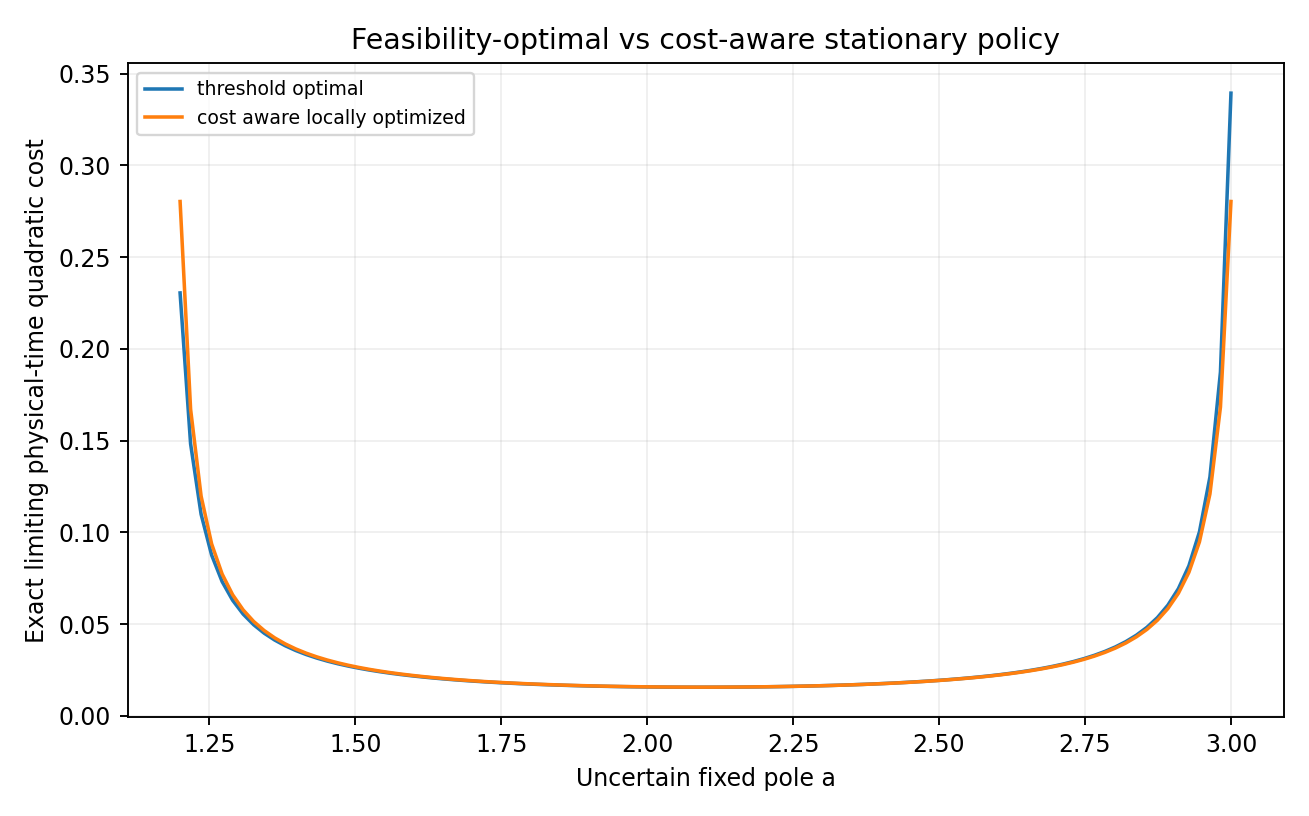
\includegraphics[width=.88\linewidth]{fig05_cost_aware_stationary.png}
\caption{Exact limiting quadratic costs from Proposition~\ref{prop:geomcost}. Both policies are stable over the full interval; the cost-aware parameters result from local grid optimization.}\label{fig:costaware}
\end{figure}

\subsection{Rate-aware weighted polynomial periodic baseline}
Fix a period $m$ and a target rate $q>1-a_2^{-2}$. Any impulse gain schedule has a monic characteristic polynomial $P_m(a)=\prod_{j=0}^{m-1}(a-c_j)$. Its exact fixed-plant second-moment contraction is
\[
\mathcal R_m(a)=\left[\frac{q}{1-ra^2}\right]^mP_m(a)^2.
\]
We numerically solve a grid approximation to the \emph{weighted monic minimax polynomial problem}
\begin{equation}\label{eq:weightedLP}
\min_{P\text{ monic, degree }m}\;\max_{a\in[a_1,a_2]}
\frac{q^{m/2}|P(a)|}{(1-ra^2)^{m/2}}.
\end{equation}
Represent $P(a)=\alpha_m T_m(t)+\sum_{j=0}^{m-1}\alpha_jT_j(t)$ with $t=(2a-a_1-a_2)/d$ and $\alpha_m=d^m/2^{2m-1}$. The finite-grid problem is a linear program in $\alpha_0,\ldots,\alpha_{m-1}$ and the maximum residual $z$; for each reported design, the recovered polynomial has
$m$ real roots, which define the periodic gains.
The corresponding computed roots are listed in
Table~\ref{tab:periodic_gains}. The certificate treats the stored binary64 gains as exact dyadic numbers. The design uses $[a_1,a_2]$ and $q$, but not the true plant. The grid optimum alone gives no continuum guarantee.

For an explicit bound, write $W(a)=[q/(1-ra^2)]^{m/2}$, $S_0=\sum_{j=0}^m|\alpha_j|$, and $S_1=\frac2d\sum_{j=1}^m j^2|\alpha_j|$. Since $|T_j(t)|\le1$ and $|T'_j(t)|\le j^2$ on $[-1,1]$,
\begin{equation}\label{eq:Lip}
\sup_{a\in[a_1,a_2]}|(WP)'(a)|\le
L:=\left[\frac{q}{1-ra_2^2}\right]^{m/2}
\left(S_1+\frac{mra_2}{1-ra_2^2}S_0\right).
\end{equation}
For a uniform grid spacing $\Delta$, any continuum point is within $\Delta/2$ of a grid point, whence
\begin{equation}\label{eq:bound}
\max_{a\in[a_1,a_2]}|W(a)P(a)|\le\max_{a\in\mathcal G}|W(a)P(a)|+\frac{L\Delta}{2}.
\end{equation}
The strict inequality in \eqref{eq:bound} with right-hand side below one certifies the selected gains over the interval. For $m=6$, $W(a)$ has integer exponent three; \texttt{src/verify\_weighted\_exact.py} recomputes the polynomial, grid values and derivative bound using rational arithmetic. The resulting certificate concerns the stored ideal gains, not an optimal solution over all periods or finite-precision actuators.


\begin{table}[t]
\centering
\caption{Computed real gains for the optimized period-six
policies. The values are rounded to six decimal places;
the stability certificates use the stored full-precision gains.}
\label{tab:periodic_gains}
\scriptsize
\setlength{\tabcolsep}{3pt}
\begin{tabular}{@{}ccrrrrrr@{}}
\toprule
$\Theta$ & $q$ & $c_1$ & $c_2$ & $c_3$ & $c_4$ & $c_5$ & $c_6$ \\
\midrule
$[1.2,3.0]$ & 0.92 &
1.244771 & 1.576902 & 2.096755 & 2.569667 & 2.860796 & 2.985588 \\
$[1.2,3.0]$ & 0.96 &
1.235368 & 1.501180 & 1.944414 & 2.417100 & 2.783858 & 2.975829 \\
$[1.5,4.5]$ & 0.98 &
1.560258 & 2.013693 & 2.768001 & 3.560261 & 4.157866 & 4.462171 \\
\bottomrule
\end{tabular}
\end{table}

\subsection{Numerical results and fairness protocol}\label{sec:experiments}


\subsection{Numerical results and fairness protocol}\label{sec:experiments}
We compare controllers under common Bernoulli arrivals, noise and initial conditions, using 1200 paired trajectories of length 300 (seed 20261020), $\sigma^2=0.01$, $x_0\sim\mathcal N(0,1)$ and $J_T=T^{-1}\sum_{k=0}^{T-1}(x_k^2+0.05u_k^2)$. The oracle uses the true pole and is therefore not implementable when $a$ is unknown. Stationary feedback may act between receptions; periodic impulse feedback acts only upon reception. We also report peak state and input magnitudes.

\begin{table}[t]\centering\small
\caption{Weighted period-six policies. Grid maxima are LP objective values; interval upper bounds are certified by rational arithmetic applied to the stored dyadic gains. A bound below one proves contraction.}\label{tab:weighted}
\begin{tabular}{@{}lrrrc@{}}\toprule
Interval & $q$ & LP grid peak & Exact interval bound & Contracting\\\midrule
$[1.2,3.0]$ & 0.92 & 0.069095 & 0.123617 & yes \\
$[1.2,3.0]$ & 0.96 & 0.028694 & 0.031186 & yes \\
$[1.5,4.5]$ & 0.98 & 0.687974 & 0.764793 & yes \\
\bottomrule\end{tabular}
\end{table}

\begin{figure}[t]\centering
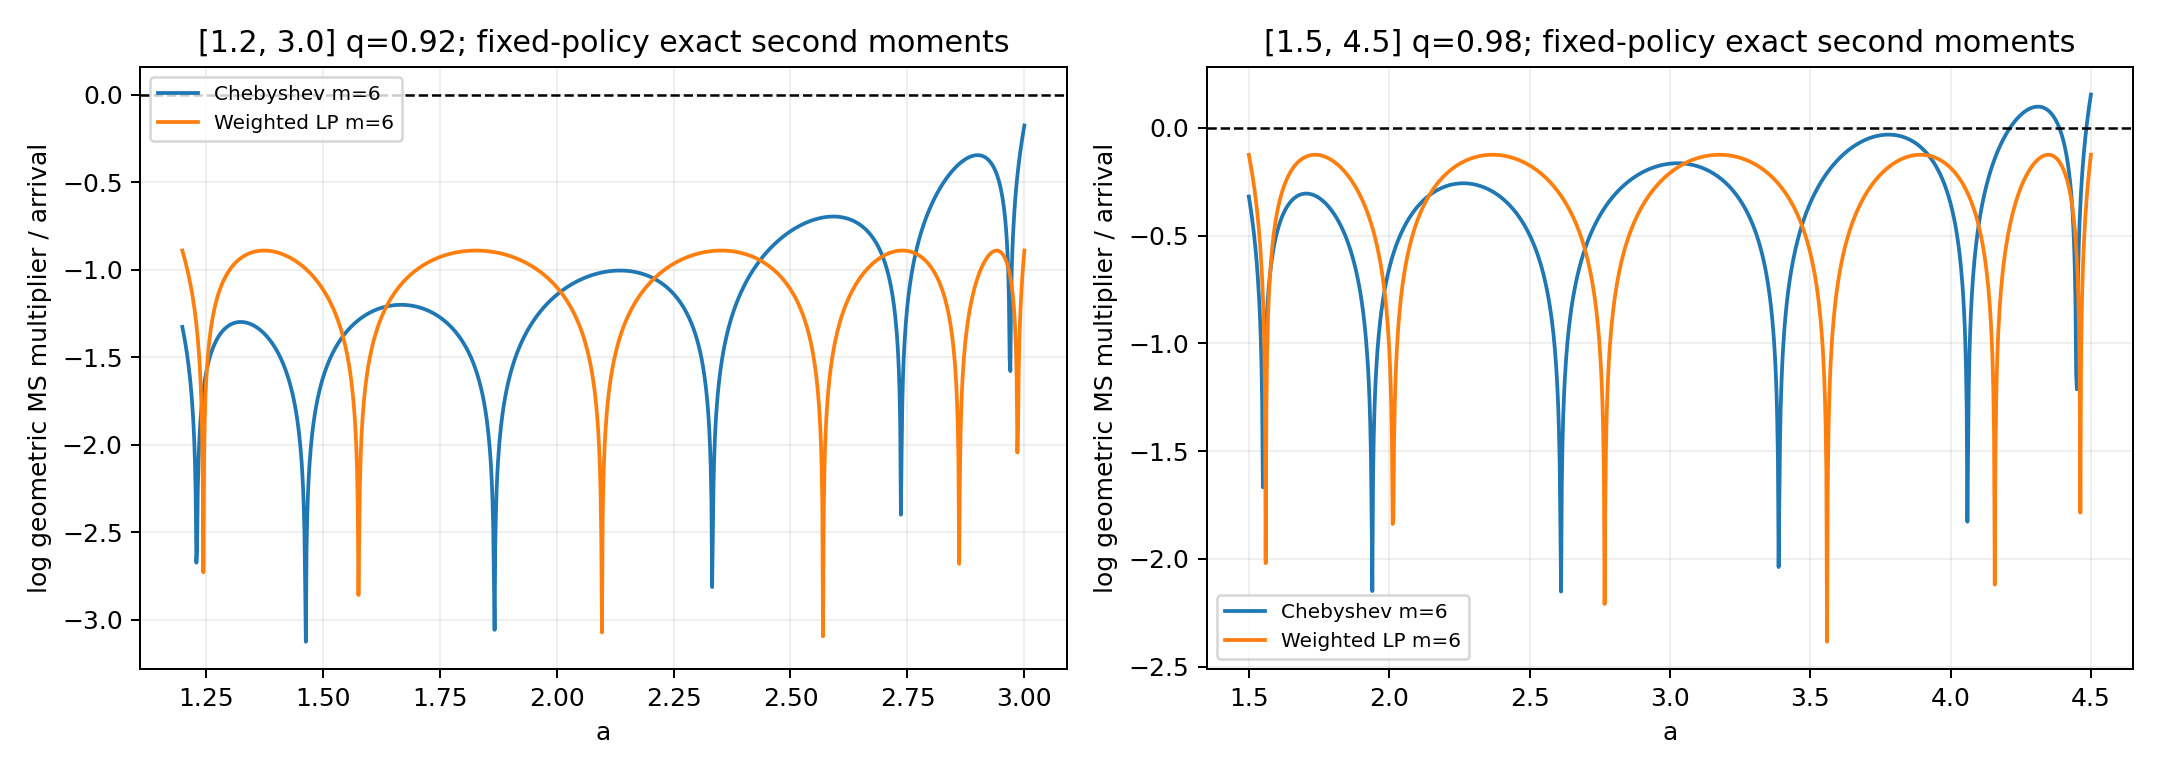
\includegraphics[width=.99\linewidth]{fig01_periodic_stability.png}
\caption{Logarithmic reception-index second-moment factors for the ordinary and weighted period-six impulse schedules. Negative values indicate contraction.}\label{fig:stability}
\end{figure}
\begin{figure}[t]\centering
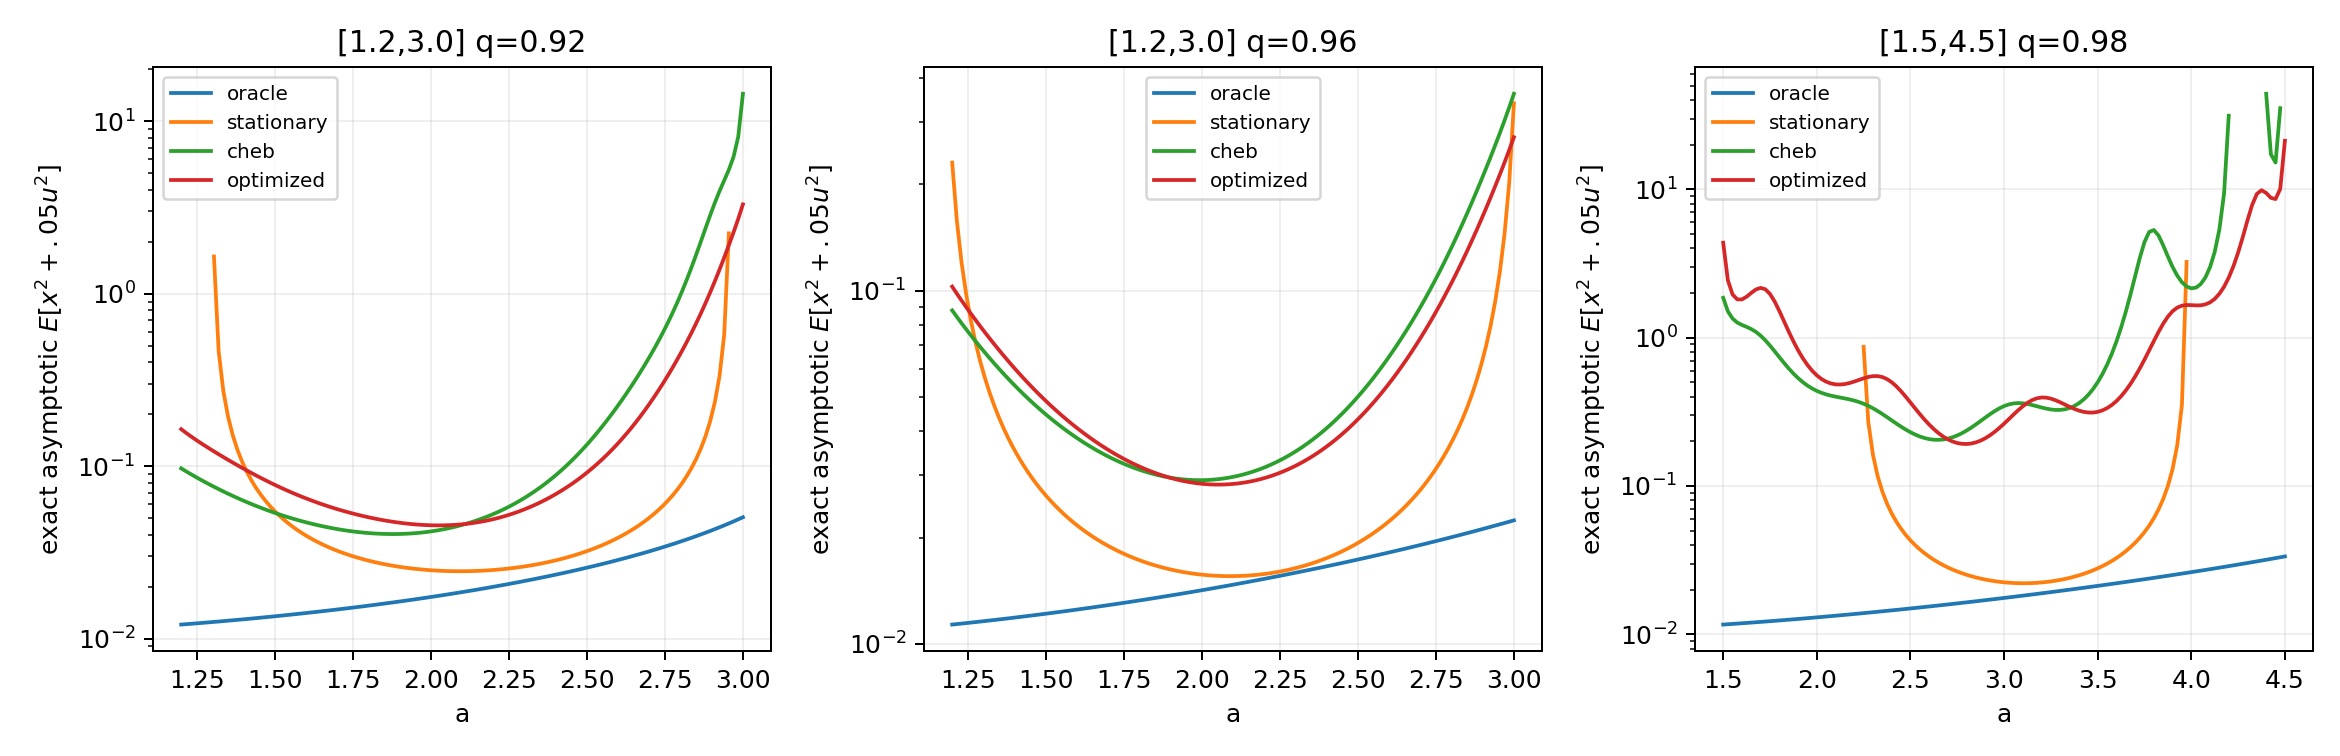
\includegraphics[width=.99\linewidth]{fig02_exact_asymptotic_costs.png}
\caption{Exact asymptotic quadratic costs where finite. Curves are omitted for plants without a finite stationary second moment.}\label{fig:costs}
\end{figure}
\begin{figure}[t]\centering
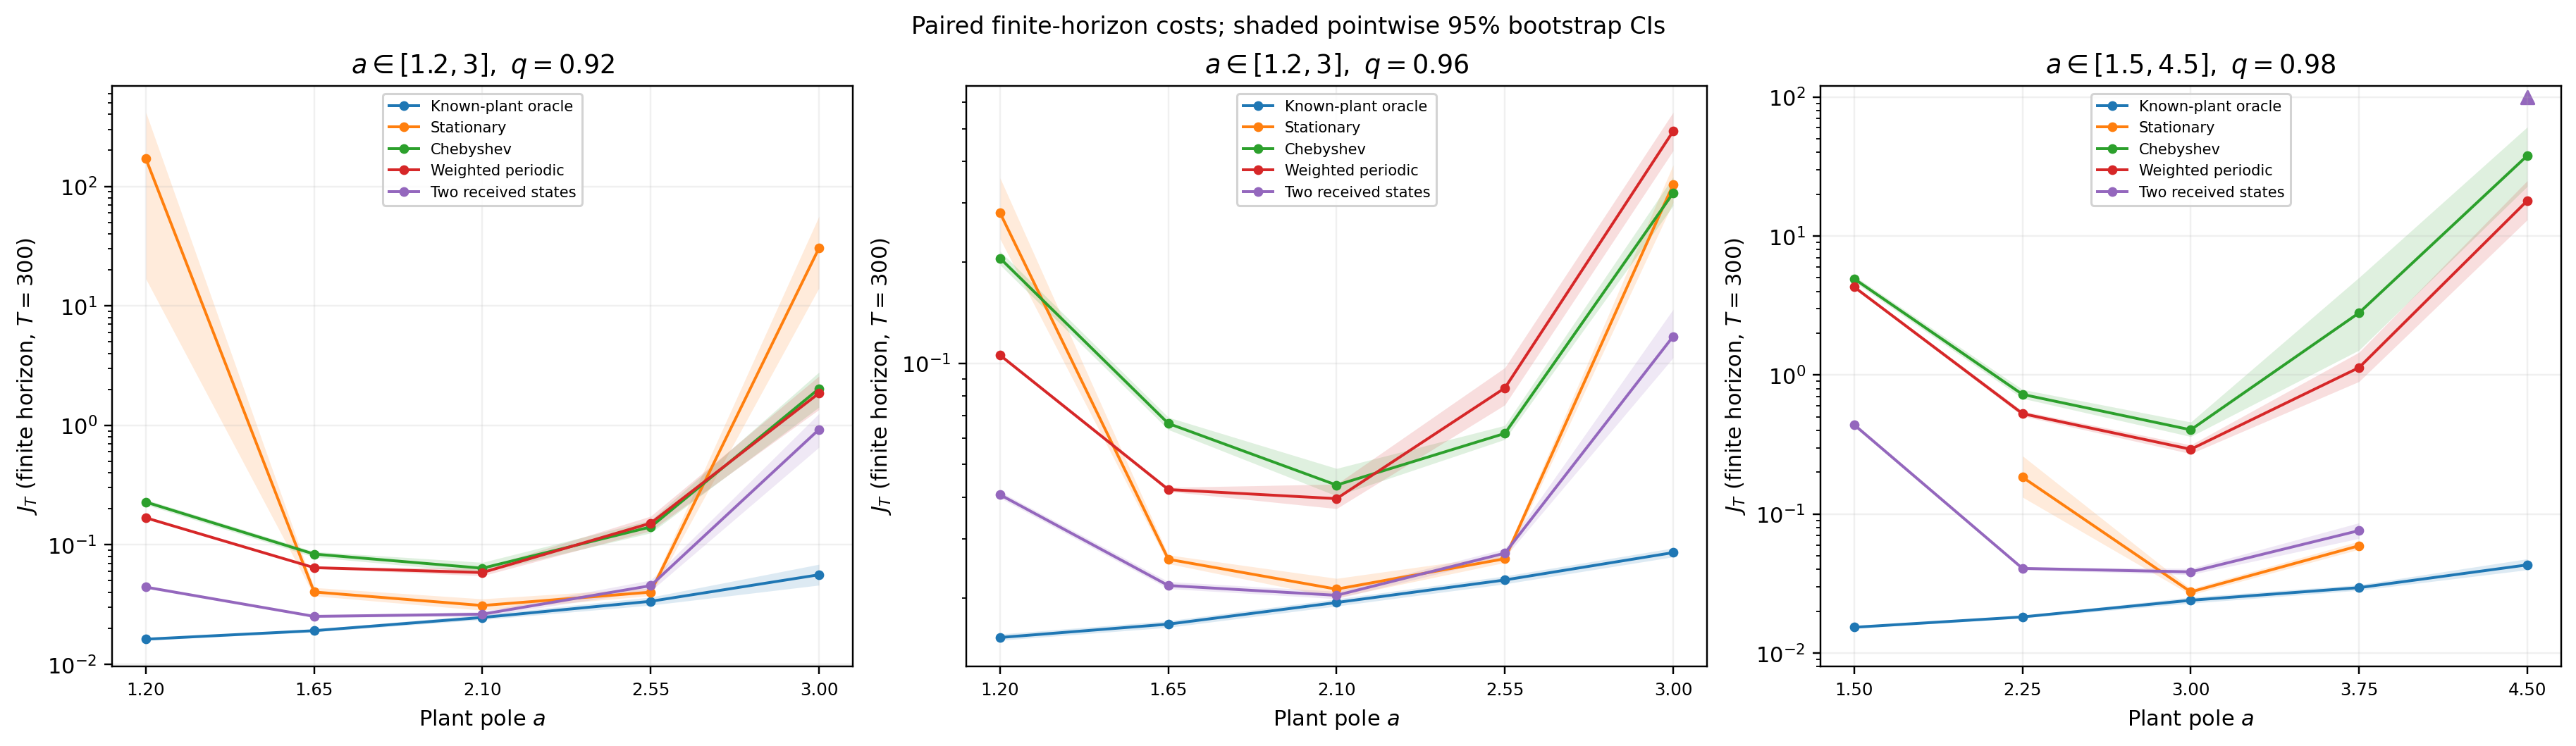
\includegraphics[width=.99\linewidth]{fig03_finite_horizon_mc.png}
\caption{Paired finite-horizon Monte Carlo mean costs ($N=1200$, $T=300$). At $q=0.98$, all policies are evaluated at five equally spaced poles, while stationary feedback is displayed only at the three interior poles because its endpoint fixed-plant second-moment multipliers exceed one. The two-received policy has a cost of $6.80\times10^4$ at $a=4.5$ (off the displayed scale, marked explicitly); such finite-horizon costs are not stability certificates.}\label{fig:mc}
\end{figure}
\begin{figure}[t]\centering
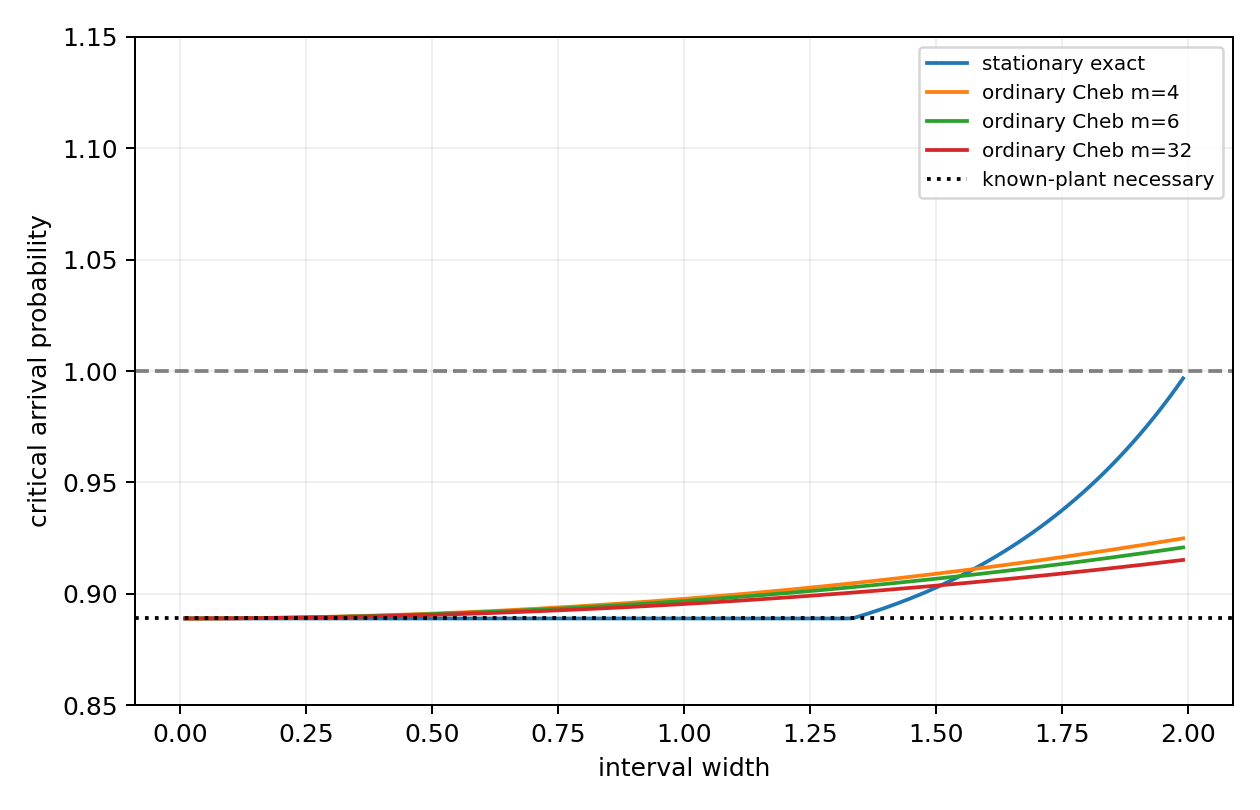
\includegraphics[width=.70\linewidth]{fig04_analytic_thresholds.png}
\caption{Critical reception rates for the stationary and ordinary-Chebyshev controller families.}\label{fig:thresholds}
\end{figure}

In Fig.~\ref{fig:mc}, the $q=0.98$ case uses five equally spaced plant values $a=1.5,2.25,3,3.75,4.5$. The stationary policy is shown only at the three interior plants; its endpoint multipliers are $2.689\ldots>1$, so its endpoint asymptotic costs are not finite. The cost-aware simulation uses 3500 paired trajectories of length 500 (seed 20261064). At $a=3$, the exact asymptotic cost decreases from $0.339402$ to $0.280345$; at $a=1.2$, it increases from $0.230494$ to $0.280345$. The design seeks to reduce the worst grid value, not the cost at each endpoint.

At $q=0.98$ on $[1.5,4.5]$, the ordinary period-six Chebyshev gains fail the worst-plant second-moment test, whereas the computed weighted period-six gains satisfy the continuum bound in Table~\ref{tab:weighted}. This is a comparison of two specified schedules at one rate. Finite-horizon costs may remain modest even when the asymptotic condition fails; only exact moment formulas are used for steady-state cost claims.

For the two-observation impulse baseline, an exact $3\times3$ reception-time moment matrix gives pointwise stability tests. Its spectral radius exceeds one at the upper endpoint in some scenarios. The numerical grid in the supplementary results does not certify the interval; Proposition~\ref{prop:cert} concerns a different, explicitly verified endpoint design.

\section{Discussion}

The stationary threshold in Theorem~\ref{thm:main} is exact under the last-received-state information restriction, not for arbitrary linear feedback. Older measurements and arrival-indexed periodic gains yield different closed-loop dynamics, as also suggested by classical periodic-compensation results \citep{khargonekar1985periodic}. Okano and Ishii \citep{okano2012lossy,okano2013,okano2014markov,okano2015} consider quantized observations, different uncertainty and channel models, and stability criteria that must not be identified with our bounded-second-moment formulation under persistent process noise. Whether the present restricted-class threshold follows from earlier robust-synthesis results remains a bibliographic question, especially in relation to \citet{elia2005,silvapulgar2011,eliaeisenbeis2011}.

The performance calculation adds a distinction often obscured by critical-rate comparisons. The gain sequence achieving the lowest admissible rate need not minimize a quadratic cost. In our numerical example, local cost optimization improves the largest exact cost on a specified plant grid, with a separate exact interval stability test. Likewise, weighted periodic gains can contract where ordinary Chebyshev gains of the same period do not. Neither computation establishes a globally optimal policy. The endpoint memory-three certificates should not be read as continuum-robustness results.


The analysis assumes a fixed scalar pole, exact received states, independent packet erasures and reliable actuation, without input saturation. In contrast, input-constrained adaptive control \citep{siriya2022}, adaptive LQR with time-varying parameters \citep{bartos2026}, and learning or predictive approaches with different channel models \citep{zhang2025,sun2025} do not provide directly matched baselines. Our numerical designs use fixed periods, local optimization and ideal dyadic gains; finite simulations alone do not certify asymptotic stability. Scripts and exact certificates are provided in the research package.



\section{Conclusions}
For stationary last-received-state feedback, we obtained a critical reception rate and a stabilizing gain schedule valid over a scalar uncertainty interval. Periodic reception-indexed policies and controllers retaining an earlier state do not obey the same class restriction. Renewal identities also give exact quadratic performance measures, which reveal a trade-off between stabilization margin and control cost. The certified examples demonstrate what the specified policies achieve; their interpretation does not extend to arbitrary feedback laws.

\paragraph{Data and code availability}
The source code, tests, numerical results and CPU notebook are supplied with the research package. A permanent repository and DOI have not yet been assigned.
\paragraph{Declaration of competing interests}
To be confirmed by the authors before submission.
\paragraph{Declaration of generative AI and AI-assisted technologies}
OpenAI ChatGPT was used to assist manuscript drafting, language revision, and the preparation and checking of research code. The authors must review and verify all material before submission and remain responsible for the final text, analyses and conclusions. Any additional tools used must be disclosed by the authors in accordance with Elsevier's policy.

\begingroup\footnotesize\begin{thebibliography}{99}
\bibitem[Sinopoli et~al.(2004)]{sinopoli2004} B.~Sinopoli, L.~Schenato, M.~Franceschetti, K.~Poolla, M.~I.~Jordan, S.~S.~Sastry. Kalman filtering with intermittent observations. \emph{IEEE Trans.\ Automat.\ Control}, 49(9):1453--1464, 2004. doi:10.1109/TAC.2004.834121.
\bibitem[Schenato et~al.(2007)]{schenato2007} L.~Schenato, B.~Sinopoli, M.~Franceschetti, K.~Poolla, S.~S.~Sastry. Foundations of control and estimation over lossy networks. \emph{Proc.\ IEEE}, 95(1):163--187, 2007.
\bibitem[Imer et~al.(2006)]{imer2006} O.~C.~Imer, S.~Y\"uksel, T.~Ba\c{s}ar. Optimal control of LTI systems over unreliable communication links. \emph{Automatica}, 42(9):1429--1439, 2006.
\bibitem[Elia(2005)]{elia2005} N.~Elia. Remote stabilization over fading channels. \emph{Systems \& Control Letters}, 54(3):237--249, 2005, doi:10.1016/j.sysconle.2004.08.009.
\bibitem[Silva and Pulgar(2011)]{silvapulgar2011} E.~I.~Silva, S.~A.~Pulgar. Control of LTI plants over erasure channels. \emph{Automatica}, 47(8):1729--1736, 2011. doi:10.1016/j.automatica.2011.02.050.
\bibitem[Elia and Eisenbeis(2011)]{eliaeisenbeis2011} N.~Elia, J.~N.~Eisenbeis. Limitations of linear control over packet drop networks. \emph{IEEE Trans.\ Automat.\ Control}, 56(4):826--841, 2011. doi:10.1109/TAC.2010.2080150.


\bibitem[Lu et~al.(2019)]{lu2019} J.~Lu, W.~Su, Y.~Wu, M.~Fu, J.~Chen. Mean-square stabilizability via output feedback for a non-minimum phase networked feedback system. \emph{Automatica}, 105:142--148, 2019. doi:10.1016/j.automatica.2019.03.001.

\bibitem[Li et~al.(2024)]{li2024} J.~Li, J.~Lu, W.~Su. Mean-square stability and stabilizability for LTI and stochastic systems connected in feedback. arXiv:2402.04074, 2024.
\bibitem[Martins et~al.(2006)]{martins2006feedback} N.~C.~Martins, M.~A.~Dahleh, N.~Elia. Feedback stabilization of uncertain systems in the presence of a direct link. \emph{IEEE Trans. Automat. Control}, 51(3):438--447, 2006. doi:10.1109/TAC.2006.871940.
\bibitem[Okano and Ishii(2012)]{okano2012lossy} K.~Okano, H.~Ishii. Data rate limitations for stabilization of uncertain systems over lossy channels. arXiv:1201.1170, 2012.
\bibitem[Okano and Ishii(2017)]{okano2015} K.~Okano, H.~Ishii. Stabilization of uncertain systems using quantized and lossy observations and uncertain control inputs. \emph{Automatica}, 81:261--269, 2017. doi:10.1016/j.automatica.2017.03.036.

\bibitem[Okano and Ishii(2014a)]{okano2014rate} K.~Okano, H.~Ishii. Minimum data rate for stabilization of linear systems with parametric uncertainties. arXiv:1405.5932, 2014.

\bibitem[Okano and Ishii(2013)]{okano2013} K.~Okano, H.~Ishii. Networked control of uncertain systems over data rate limited and lossy channels. \emph{IEICE Trans. 
Fundamentals}, E96-A(5):853--860, 2013. doi:10.1587/transfun.E96.A.853.

\bibitem[Okano and Ishii(2014b)]{okano2014markov} K.~Okano, H.~Ishii. Stabilization of uncertain systems with finite data rates and Markovian packet losses. \emph{IEEE Trans. Control Netw. Syst.}, 1(4):298--307, 2014. doi:10.1109/TCNS.2014.2338572.

\bibitem[Ding et al.(2026)]{ding2026} X.~Ding, Y.~Zhang, J.~Xue, J.~Zhou. Mean-square exponential ultimate boundedness of networked control systems with packet-loss-adaptive event triggering and scale-normalized encoding. \emph{Electronic Research Archive}, 34(11):8689--8718, 2026. doi:10.3934/era.2026366.


\bibitem[Tannenbaum(1980)]{tannenbaum1980} A.~Tannenbaum. Feedback stabilization of linear dynamical plants with uncertainty in the gain factor. \emph{Int.\ J.\ Control}, 32(1):1--16, 1980. doi:10.1080/00207178008922838.


\bibitem[Khargonekar et~al.(1985)]{khargonekar1985periodic} P.~P.~Khargonekar, K.~Poolla, A.~Tannenbaum. Robust control of linear time-invariant plants using periodic compensation. \emph{IEEE Trans.\ Automat.\ Control}, 30(11):1088--1096, 1985. doi:10.1109/TAC.1985.1103841.

\bibitem[Wu et~al.(2026)]{wu2024} W.~Wu, J.~Chen, M.~R.~Jovanovi\'c, T.~T.~Georgiou. Tannenbaum's gain-margin optimization meets Polyak's heavy-ball algorithm. \emph{IEEE Trans. Automat. Control}, 71(9):5817--5832, 2026. doi:10.1109/TAC.2026.3678501.



\bibitem[Song et~al.(2026)]{song2026} J.~Song, Z.~Wang, Q.~Liu, X.~He. Remote state estimation over hidden Markov channels: Handling measurement compression and channel-state-dependent packet loss. \emph{Automatica}, 188:112925, 2026. doi:10.1016/j.automatica.2026.112925.



\bibitem[Cui and Lindquist(2024)]{cui2024} Y.~Cui, A.~Lindquist. A general solution to the simultaneous stabilization problem by analytic interpolation. arXiv:2405.13440, 2024.

\bibitem[Siriya et~al.(2023)]{siriya2022} S.~Siriya, J.~Zhu, D.~Ne\v{s}i\'c, Y.~Pu. Learning-based adaptive control for stochastic linear systems with input constraints. \emph{IEEE Control Syst. Lett.}, 7:1273--1278, 2023. doi:10.1109/LCSYS.2022.3232692.

\bibitem[Zhang et~al.(2025)]{zhang2025} Z.~Zhang, L.~Xu, Y.~Mo, X.~Wang. Learning control for LQR with unknown packet loss rate using finite channel samples. arXiv:2501.02899, 2025.
\bibitem[Costa et~al.(2005)]{costa2005} O.~L.~V.~Costa, M.~D.~Fragoso, R.~P.~Marques. \emph{Discrete-Time Markov Jump Linear Systems}. Springer, 2005.

\bibitem[Duren(1970)]{duren1970} P.~L.~Duren. \emph{Theory of $H^p$ Spaces}. Academic Press, 1970.

\bibitem[Chen and Li(2023)]{chen2023} W.~Chen, X.~Li. Data-driven control for networked systems with multiple packet dropouts. \emph{Int. J. Robust Nonlinear Control}, 33(12):7357--7373, 2023. doi:10.1002/rnc.6754.
\bibitem[Lu et~al.(2025)]{lu2025} J.~Lu, J.~Li, W.~Su. Mean-square input-output stability and asymptotic stationarity of networked control systems with random transmission delays. \emph{Automatica}, 178:112339, 2025. doi:10.1016/j.automatica.2025.112339.
\bibitem[Sun et~al.(2025)]{sun2025} H.-Y.~Sun, H.-R.~Mu, S.-J.~Fu, H.-G.~Han. Data-driven model predictive control for unknown nonlinear NCSs with stochastic sampling intervals and successive packet dropouts. \emph{IEEE Trans. Cybern.}, 55(6):2899--2909, 2025. doi:10.1109/TCYB.2025.3555766.
\bibitem[Bartos et~al.(2026)]{bartos2026} M.~Bartos, J.~K\"ohler, F.~D\"orfler, M.~N.~Zeilinger. Stability of certainty-equivalent adaptive LQR for linear systems with unknown time-varying parameters. \emph{Proc. Mach. Learn. Res.}, 331:1363--1381, 2026.
\end{thebibliography}\endgroup
\end{document}
